\chapter{El Sistema de Televisión Digital Terrestre ISDB-T}

El esquema de transmisión del estándar ISDB-T que se presenta en la Figura \ref{f:esquema-tx} puede ser caracterizado en cuatro grandes etapas que serán presentadas en este capítulo: el flujo de transporte BTS (\textit{Broadcast Transport Stream}), la etapa de robustecimiento de la señal, la formación de los Cuadros OFDM con sus señales piloto y la puesta en el aire de la señal.

\begin{figure}[h!]
	\centering
	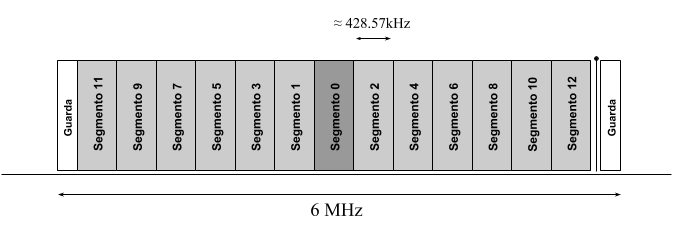
\includegraphics[scale=0.55]{figuras/cap03/segmentos_isdbt}
	\caption{\label{segmentos_isdbt} Distribuci\'on espectral de los segmentos OFDM. A la derecha, entre el segmento 12 y el intervalo de guarda, puede apreciarse la presencia del piloto continuo.}
\end{figure}

Cada una de esas etapas tiene a su vez varias subetapas, o bloques fundamentales, que se enfocan en resolver los distintos problemas discutidos que surgen al transmitir una señal inalámbrica. Esto dá como resultado una variedad de parámetros de operación presentados en la Tabla \ref{parametros_ISDBT} que permitirán por ejemplo, la transmisión jerárquica en distintas capas, cada una con su propia configuración; o enfocarse en robustecer la transmisión frente al \textit{multipath} o al efecto Doppler.

A nivel de la distribuci\'on en el espectro, el estándar utiliza 6 MHz de ancho de banda de canal distribu\'ido en 14 segmentos de los cuales sólo 13 son utilizados para enviar datos, el restante se utiliza como guarda a ambos lados del canal. Tambi\'en se incluye un piloto continuo que se trata de una portadora modulada en BPSK ubicada a continuaci\'on del Segmento 12.

Tener un esquema de transmisi\'on jer\'arquica permite asignar a cada capa jer\'arquica la cantidad de segmentos que uno quiera. El est\'andar de la ARIB denomina a estas capas como A, B y C, y es posible tener configurac\'ones con solamente 2 capas presentes tal como la de la Figura \ref{segmentos_isdbt} en la que la capa A corresponde al segmento 0 y el resto de los segmentos forman la capa B.

En los comienzos de la televisi\'on digital en el Uruguay los operadores que prestaban servicios de televisi\'on digital deb\'ian transmitir su señal en calidad HD, en SD y \textit{oneseg}, es decir en tres capas jer\'arquicas. Esto era as\'i porque se entend\'ia que en el mercado circulaba una gran cantidad de receptores que no eran capaces de procesar la calidad HD. Posteriormente esa directiva fu\'e suprimida y al d\'ia de hoy los operadores no est\'an obligados a transmitir en SD.

El sistema puede operar en tres \textit{modos de transmisi\'on} diferentes que se caracterizan por la cantidad de portadoras utilizadas, siempre en el mismo ancho de banda de 6 MHz. Las portadoras utilizadas son $2^{10+modo}$ donde el modo puede ser 1, 2 o 3.

Se define la frecuencia de muestreo de la IFFT como $f_{IFFT} \triangleq \frac{512}{63 \mu s} \approx 8.127 MHz$, que a su vez coincide con el n\'umero de portadoras utilizadas sobre el tiempo de s\'imbolo activo $T_s$. Por lo tanto la utilizaci\'on de un n\'umero mayor de portadoras implica utilizar s\'imbolos m\'as largos para respetar la relaci\'on de la $f_{IFFT}$; aumentar el tiempo de s\'imbolo activo implica reducir el ancho de banda ocupado por cada portadora.

Cada segmento a su vez est\'a conformado por dos tipos de señales portadoras. Las primeras son las correspondientes a los datos, y las otras son las denominadas \textit{portadoras piloto} que cumplen se utilizan para la estimaci\'on del canal y transmisi\'on de par\'ametros de control e informaci\'on del sistema.
De manera general, los segmentos tienen $96 \times 2^{modo-1}$ portadoras de datos $12 \times 2^{modo-1}$ portadoras piloto dependiendo del modo de transmisi\'on. En la Tabla \ref{parametros_ISDBT} se eval\'uan estos par\'ametros para los distintos modos de transmisi\'on. 


\begin{figure}[h!]
\centering
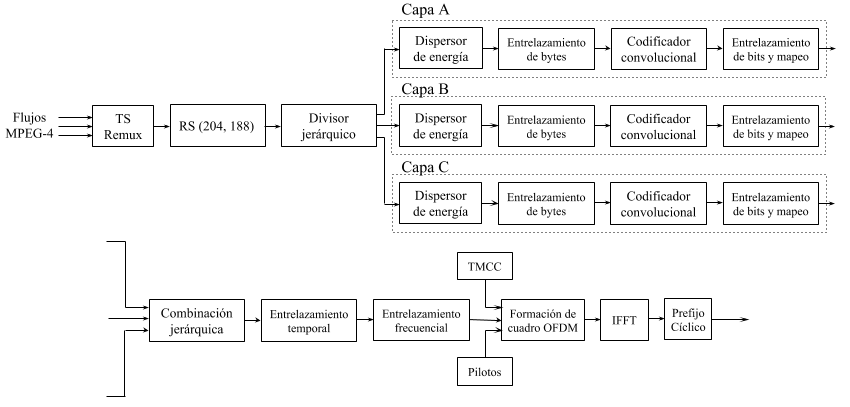
\includegraphics[scale=0.5]{figuras/cap03/esquema-tx}
\caption{\label{f:esquema-tx} Diagrama de bloques del transmisor ISDB-T definido por la ARIB.}
\end{figure}


\begin{table}[h!]
\centering
\begin{tabular}{|c|c|}
\hline
\textbf{Parámetro} 				& \textbf{Valor}\\
\hline
Ancho de banda del canal 		& 6 MHz\\
\hline
Cantidad de segmentos 			& 13 \\
\hline
Ancho de banda de cada segmento & $6000/14 \approx 428.57kHz$ \\
\hline
  											& 96 de datos y 12 pilotos (Modo 1) \\
Cantidad de portadoras activas por segmento & 192 de datos y 24 pilotos (Modo 2) \\
 											& 384 de datos y 48 pilotos (Modo 3)\\
\hline
 								& $252 \mu s$ (Modo 1)\\
Duración de símbolo activo 		& $504 \mu s$ (Modo 2) \\
								& $1008 \mu s$ (Modo 3) \\
\hline
Duracion del prefijo ciclico 	& 1/4, 1/8, 1/16, 1/32 \\
 								& (fraccion del simbolo activo)\\
\hline
Tasa de codigo convolucional 	& 1/2, 2/3, 3/4, 5/6, 7/8\\
\hline
Tasa de codigo Reed-Solomon 	& (188, 204) \\
\hline
 								& 0, 1, 2, 4 (Modo 1) \\
Profundidad del entrelazamiento temporal & 0, 2, 4, 8 (Modo 2) \\
 & 0, 4, 8, 16 (Modo 3)\\
\hline
Esquemas de modulacion & DQPSK, QPSK,\\
 & 16QAM, 64QAM\\
 \hline
 Frecuencia de muestreo ($f_{IFFT}$) & 512/63 $\approx$ 8.127 MHz\\
 \hline
\end{tabular}
\caption{\label{parametros_ISDBT} Par\'ametros relevantes en el est\'andar ISDB-T.}
\end{table}



\section{BTS como fuente de datos}

El est\'andar ISDB-T admite la posibilidad de tomar hasta tres \textit{Transport Streams} (TS) MPEG-4. A estos flujos se les debe agregar la informaci\'on necesaria para la transmisi\'on en capas jer\'arquicas. El bloque TS Remux es el que se encarga de multiplexar los tres flujos de transporte y a cada TSP agregarle 16 bytes de informaci\'on. 
Una vez que se agregan estos datos los paquetes de cada capa son multiplexados seg\'un un patr\'on de ordenamiento que es \'unico para cada configuraci\'on del sistema, en \cite{multiplex-pattern} se explica este patr\'on y se presenta un algoritmo para recuperarlo en recepci\'on. El transmisor implementado en este trabajo toma como flujo de entrada un BTS ya conformado, y con la informaci\'on jer\'arquica de los TSP es que logra procesar cada capa por separada. De ah\'i en adelante las capas son entrelazadas y moduladas cada una de acuerdo a su propia configuraci\'on. 

\section{Robustecimiento frente a las no idealidades del canal}

Como primer medida para proteger los datos del BTS se aplica un c\'odigo Reed-Solomon (204, 188). El proceso de codificaci\'on consiste en sustituir los \'ultimos 16 bytes de los TSP por una paridad que permite corregir hasta 8 bytes de error en el paquete. 

Este bloque remueve la informaci\'on jer\'arquica agregada por el TS Remux con lo cual una vez que los TSP son codificados por el Reed-Solomon en principio ya no es posible distinguir a qu\'e capa pertenece cada paquete, es decir que al llegar al bloque de divisi\'on jer\'arquica ya no se cuenta con esa informaci\'on. Una estrategia para sortear este problema, y de hecho la que se implementa en \textit{gr-isdbt-tx}, consiste en separar primero los paquetes correspondientes a cada capa jer\'arquica y luego codificar los paquetes. Una vez encaminados los paquetes se puede prescindir de la informaci\'on jer\'arquica. El diagrama de bloques presentado en la Figura \ref{f:esquema-tx} corresponde al esquema original de la ARIB en la que se define el est\'andar ISDB-T, mientras que la Figura \ref{f:esquema-tx} se encuentra la implementaci\'on utilizada en \textit{gr-isdbt-tx}. 

% Dispersor de energia
Para evitar los problemas de sincronismo que podr\'ia ocasionar una se\'al con muchos ceros o unos consecutivos, se utiliza un \textit{dispersor de energ\'ia} que se encarga de generar un flujo pseudoaleatorio. Este proceso se define de manera tal que resulta ser totalmente invertible y por lo tanto aplicando el mismo proceso en recepc\'ion se obtiene la secuencia original.



% Entrelazamiento
Los canales inal\'ambricos son propensos a una multiplicidad de fuentes de error. Un tipo de errores muy comunes en estos canales son los \textit{errores en r\'afaga} provocando que una secuencia consecutiva de bits se corrompan. El impacto de estos tipos de errores crece con la velocidad de transmisi\'on; a mayor velocidad de transmisi\'on un mismo error afecta a una mayor cantidad de bits.
Resulta necesario lograr alg\'un tipo de inmunidad ante estos errores, es por ello que en muchos sistemas, y en particular en ISDB-T, se suelen concatenar c\'odigos correctores de errores. David Forney en su trabajo \textit{Concatenated Codes} \cite{forney1965concatenated} estudia el compromiso que existe en la utilizaci\'on de sucesivos c\'odigos concatenados, y en especial la performance que pueden llegar a alcanzar los c\'odigos Reed-Solomon concatenados.
El est\'andar ISDB-T utiliza este enfoque a trav\'es de la implementaci\'on de un c\'odigo Reed-Solomon como \textit{outer code} y un c\'odigo convolucional como \textit{inner code}.
Como medida adicional para contrarrestar los efectos del canal se utiliza el \textit{entrelazamiento de bits} que esencialmente consiste en introducir retardos variables en los bits que se transmiten.

Al transmitir en m\'ultiples portadoras ortogonales se corre el riesgo de atravesar canales selectivos en frecuencia y por lo tanto que ciertas portadoras se vean continuamente afectadas. Para mitigar esto una estrategia puede ser rotar de portadora los contenidos que se transmiten, es decir hacer un \textit{entrelazamiento frecuencial}. Con esto se logra que ante un canal selectivo, ya lo sea por sus caracter\'isticas propias o por interferencias de señales espurias fuera de banda, las portadoras que son afectadas no resulte en una p\'erdida de bloques de informaci\'on irrecuperables.


\section{Formacion de los cuadros OFDM}

El estándar define una estructura de cuadro OFDM formada por un conjunto de 204 símbolos OFDM consecutivos, es decir que, por ejemplo, para el modo 1 se tienen 108 símbolos complejos por segmento con lo cual un cuadro OFDM en modo 1 está compuesto por $108 \times 13 \times 204$ complejos. Esta estructura facilita las tareas de sincronización en el receptor.


\section{Las portadoras y la modulacion}

Cada segmento OFDM está conformado por una cantidad de portadoras en función del modo de transmisión. La mayor cantidad de portadoras está destinada a la transmisión de los datos mientras que algunas otras son utilizadas como mecanismos para la estimación del canal, sincronización, transmisión de parámetros de funcionamiento entre otros.



Scattered Pilot
Las portadoras piloto son señales moduladas en BPSK que se generan a partir de una secuencia pseudoaleatoria PRBS (Pseudo Random Binary Sequence). El procedimiento para generar estas portadoras consiste en evolucionar el circuito de la Figura XX y tomar Wi para la modulación BPSK. El índice de la portadora SP dentro del símbolo OFDM es el que determina la cantidad de veces que se debe evolucionar el registro para obtener $W_i$.
Por último la modulación se realiza como $(4/3, 0)$ si $W_i = 0$, y $(-4/3, 0)$ si $W_i = 1$.

Las SP se ubican cada 12 portadoras y a medida que transucrren los símbolos OFDM las mismas van rotando $3 \times n MOD 4$, donde $n$ es el número de símbolo OFDM. Esto sucede así puesto que la función de estas portadoras es justamente la estimación del canal y por lo tanto para contemplar la situación de todo el canal de 6MHz es necesario ir rotándolas. 


% Circuito generador y portadoras

Portadora TMCC
Las portadoras TMCC son las que transportan toda la información de las capas jerárquicas y la información de control. Si bien en los cuadros OFDM se transmiten varias TMCC estas tienen exactamente el mismo contenido, lo que da al receptor la posibilidad de ponderar todas las TMCC que recibe para quedarse con las que tienen mayor porcentaje de coincidencia entre sí.
Se compone de 204 bits modulados en DBPSK de los cuales el primero es un bit de referencia para realizar la modulación diferencial. Este bit coincide con el valor de la $W_i$ correspondiente al primer símbolo del cuadro OFDM.
Los siguientes 16 bits son utilizados por una señal de sincronismo que puede tomar los valores $w_0 = 0011010111101110$ y $w_1 = 1100101000010001$, alternándose entre una y otra en cada cuadro OFDM.
A continuación se encuentran los datos de la información jerárquica y otros parámetros para los que se dedican 105 bits. Estos 105 bits son protegidos por un código cíclico acortado (200,118) con lo cual se dedican los siguientes 82 bits para la paridad. 
  
Portadoras Auxiliares

Las portadoras auxiliares están pensadas para transmitir información complementaria del control de transmisión. Utilizan modulación diferencial DBPSK con referencia $W_i$ al igual que la TMCC. Su uso es opcional y el sistema puede trabajar perfectamente prescindiendo de ellas; en caso de no ser usadas los bits correspondientes a las portadoras AC se rellenan con "1".

Piloto Continuo
Al igual que las SP, se agrega un piloto continuo a la derecha del segmento 12 con propósitos de sincronismo en recepción. Su modulación también es BPSK y toma el valor de $(-4/3, 0)$, $(4/3, 0)$, $(4/3, 0)$ para los modos 1, 2 y 3 respectivamente.


\section{La puesta en el aire de la señal}

Luego de conformarse el cuadro OFDM los datos ya están listos para ser transmitidos mediante la modulación OFDM. En este punto los símbolos son procesados por el bloque de la IFFT y a continuación es necesario agregar el prefijo cíclico. Una vez agregado el prefijo las muestras ya estan prontas para ser dirigidas al conversor D/A para la transmisión en ondas EM.

\subsection{Necesidad del prefijo cíclico}

Cuando se pasa de trabajar en el dominio continuo al dominio discreto muchas cosas no funcionan igual. Si bien es cierto que en el dominio continuo la transformada de Fourier de un producto convolución coincide con la transformada de cada factor, esto deja de ser válido en tiempo discreto; si $y[n] = x[n]\ast h[n] \Rightarrow DFT \left\{ y[n] \right\} \neq X[q]H[q]$.
Sería bueno poder tener una relación similar a la que ocurre en tiempo continuo y así poder separar fácilmente las muestras que se enviaron de la respuesta del canal. 

Afortunadamente existe un tipo de producto convolución especial llamado \textit{convolución circular} que nos devuelve esa propiedad de la transformada de Fourier.
Supongamos que la señal que enviamos es $x[n]$ y la respuesta del canal $h[n]$ con $n = 0,..,N-1$. La convolución circular de dos señales $x[n]$ y $h[n]$ se define de la siguiente manera:

\begin{equation}
x[n] \circledast h[n] = \sum_{k = 0}^{N-1} x[(n-k) \enskip MOD \enskip N]h[k]
\end{equation} 

Para evitar sobrecargar la notación se suele utilizar la siguiente nomenclatura $x_N[n-k] \triangleq x[(n-k) \enskip MOD \enskip N]$. Con lo cual la convolución circular queda expresada:

\begin{equation}
x[n] \circledast h[n] = \sum_{k = 0}^{N-1} x_N[n-k] h[k]
\end{equation} 

La señal $x_N[n-k]$ no es otra cosa que la señal $x[n-k]$ periodizada cada $N$ muestras. Tomemos la transformada discreta de Fourier de esta convolución circular y veamos lo que sucede.

\begin{equation}
Y[q] \triangleq DFT\left\{x[n] \circledast h[n]\right\} = \sum_{n=0}^{N-1}e^{-j2\pi \frac{ nq}{N}} \sum_{k = 0}^{N-1}x_N[n-k]h[k] 
\end{equation}

\begin{equation}
Y[q] = \sum_{k = 0}^{N-1}h[k] \sum_{n=0}^{N-1} e^{-j2\pi \frac{nq}{N}} x_N[n-k]
\end{equation}

Renombrando la variable $m$ como $n - k$ se tiene:

\begin{equation}
Y[q] = \sum_{k = 0}^{N-1}h[k] \sum_{m = -k}^{N-1-k} e^{-j2\pi (m+k)\frac{q}{N}} x_N[m]
\end{equation}

Todo lo que no depende de $m$ en la segunda sumatoria puede salir como factor

\begin{equation}\label{e:convolucion}
Y[q] = \sum_{k = 0}^{N-1}e^{-j2\pi \frac{mq}{N}}h[k] \sum_{m = -k}^{N-1-k} e^{-j2\pi \frac{mq}{N}} x_N[m]
\end{equation}

En la ecuación \ref{e:convolucion} puede apreciarse que la sumatoria en $k$ corresponde a la $DFT\left\{ h[k] \right \}$.
La otra sumatoria resulta un poco más complicado de verla pero pensemos que $x_N[m]$ es la señal $x[m]$ de $N$ muestras periodizada; la sumatoria se lleva a cabo en una ventana de $N$ muestras por lo cual esto coincide con la transformada discreta de Fourier de la señal $x[n]$. Dicho de otra manera, la sumatoria de la ecuación \ref{e:convolucion} es una manera de calcular la DFT en la que se suman los términos en otro orden, pero al final la suma es la misma.

Con esto queda demostrado que la DFT de la convolución circular de dos señales coincide con el producto de sus transformadas discretas, es decir que $DFT\left\{ h[n] \circledast x[n] \right \} = H[q]X[q]$.

Pasemos a ver qué sucede con la señal OFDM cuando se propaga por el canal inalámbrico. En principio el canal podría variar con el tiempo, con lo cual el modelo discreto de la señal recibida queda de la siguiente manera:

\begin{equation}
r[n] = \sum_{k = -\infty}^{\infty} h_k[n]x[n-k] + w[n]
\end{equation}

Donde $w[n]$ corresponde al ruido gaussiano aditivo que introduce el canal, y $h_k[n]$ es la respuesta al impulso del canal que en principio puede ser una función del tiempo. Para el estudio que realizaremos se asumirá que el canal es un sistema lineal invatiante en el tiempo y su respuesta está definida por $L$ muestras, con lo cual se elimina la dependencia de $n$:

\begin{equation}
r[n] = \sum_{k = 0}^{L-1} h_k x[n-k] + w[n]
\end{equation}

La señal resultante tendrá $N+L-1$ dado el efecto que tienen las muestras de la respuesta al impulso del canal. Esto hace que al enviar dos símbolos OFDM consecutivos haya un solapamiento de $L-1$ muestras en recepción. Como primera medida podría separarse los símbolos enviados la cantidad de muestras necesarias, sin embargo existe otra solución que consiste en el agregado de un \textit{prefijo cíclico}. La idea es utilizar esos $L$ espacios para transmitir las últimas $L$ muestras del símbolo siguiente tal como se muestra en la Figura \ref{f:prefijo_ciclico}.



El estándar ISDB-T ofrece la posibilidad de utilizar distintos largos de prefijo cíclico. Una manera de establecer sincronismo, y también poder conocer los parámetros básicos de transmisión desde el lado del receptor como el modo y el largo del prefijo cíclico, consiste en tomar símbolos OFDM consecutivos que van arribando y retardarlos una cierta cantidad de símbolos. Luego se calcula una función de verosimilitud propuesta por Van de Beek en \cite{van1997ml} y según su característica es que se puede determinar el largo del prefijo cíclico y el modo de transmisión.  

La nueva señal conformada a partir de $x[n]$ con su prefijo cíclico queda expresada de la siguiente manera:

\begin{equation}
 u[m] =
  \begin{cases}
    x[N-L+m+1]       & \quad \text{si } m = 0,..., L-2\\
    x[m-L+1]  & \quad \text{para } m = L-1,..., N+L-2
  \end{cases}
\end{equation}

Ahora con esta nueva señal que hemos definido, en recepción llegará la siguiente señal:

\begin{equation}\label{eq:pref_convolucion}
v[n] = \sum_{k = 0}^{L-1}h[k]u[n-k] + w[n] = \sum_{k = 0}^{L-1}h[k]x[n-L-k] + w[n]
\end{equation}

La superposición de las primeras $L-1$ de $v$ hace que deban descartarse. Por lo tanto se considerarán las muestas con $n = L,..., L+N-1$ y entonces es posible considerar un $n'$ el cual contempla que las muestras indicadas ya han sido descartadas. Como este es un proceso cíclico símbolo a símbolo, la ecuación \ref{eq:pref_convolucion} queda así: 

\begin{equation}
v[n'] = \sum_{k = 0}^{N-1}h[k]x_N[n'- k] + w[n'] \text{ con } n' = [0, ..., N-1]
\end{equation}

Esta última ecuación no es otra cosa que la convolución circular $h \circledast x$ y que, como se vió anteriormente, su transformada de Fourier resulta ser $Y[q] = H[q]X[q]$.
De esta manera el receptor una vez que realizó su estimación del canal es capaz de separar las muestras $X[q]$ y así recuperar la señal transmitida.

\subsection{La potencia requerida para transmitir}
- Relación entre la potencia necesaria segun la modulación
- SNR Necesario para decodificar
